\documentclass[a4paper]{article}

%% Language and font encodings
\usepackage[english]{babel}
\usepackage[utf8x]{inputenc}
\usepackage[T1]{fontenc}

%% Sets page size and margins
\usepackage[a4paper,top=3cm,bottom=3cm,left=3cm,right=3cm,marginparwidth=1.75cm]{geometry}

%% Useful packages
\usepackage{graphicx}
\usepackage{url}
\usepackage[colorlinks=true, allcolors=blue]{hyperref}
\usepackage{amsfonts}
\usepackage{amsmath}
\usepackage{physics}
\usepackage{amssymb}
\usepackage{mathtools}

\numberwithin{equation}{subsection}
\newcommand{\mb}[1]{\mathbf{#1}}
\title{Surface Plasmonic Polaritons}
\author{Kosala Sananthana Herath}
\numberwithin{equation}{section}

\begin{document}

\maketitle

\section*{Derivation of the Dispersion Equation}

Surface plasmon polaritons (SPPs) are electromagnetic waves that travel along a metal–dielectric, practically in the infrared or visible-frequency. The term "surface plasmon polariton" explains that the wave involves both charge motion in the metal ("surface plasmon") and electromagnetic waves in the air or dielectric ("polariton").

Starting the SPPs in a metal–dielectric interface know as excitation. SPPs can be excited by both electrons and photons. Excitation by electrons is created by firing electrons into the bulk of a metal. As the electrons scatter, energy is transferred into the bulk plasma. The component of the scattering vector parallel to the surface results in the formation of a SPP. For a photon to excite an SPP, both must have the same frequency and momentum. However, for a given frequency, a free-space photon has less momentum than an SPP because the two have different dispersion relations. Nevertheless, coupling of photons into SPPs can be achieved using a coupling medium such as a prism or grating to match the photon and SPP wave vectors.
\begin{figure}[ht!]
  \centering
  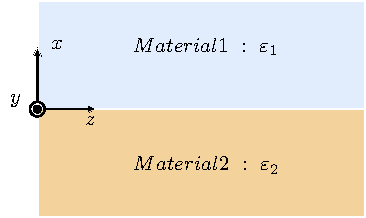
\includegraphics{figures/fig1}
  \caption{The SPPs exist on the interface of two different materials. Our considering surface is positioned in on the $yz$-plane.}
\end{figure}


Here we are goin to find electromagnetic wave solutions ($\vb{E}(x,y,z,t),\vb{H}(x,y,z,t)$) that can be exist on the metal–dielectric interface. We represent the electric field of the SPP using $\vb{E}$ and the magnetic field with $\vb{H}$. In this case, we hoping to find solutions with following properties:
\begin{itemize}
  \item Wave solutions propagte through the surface (we assume they propagate to $z$-direction) \\
  \begin{equation} \nonumber
    \vb{E} \approx e^{-i\omega t + ik_z z} \quad
    \text{and} \quad
    \vb{H} \approx e^{-i\omega t + ik_z z}.
  \end{equation}
  \item Wave solutions decay through the both mediums (in the perpendicular direction to the surface) \\
  \begin{equation} \nonumber
    \vb{E} \rightarrow 0 \quad
    \text{and} \quad
    \vb{H} \rightarrow 0 \quad
    \text{as} \quad
    x \rightarrow \pm \infty
  \end{equation}
\end{itemize}

Without loss of generality, we can assume that $|\vb{H}|$ and $|\vb{H}|$ are independent on $y$. Now we can find the solutions for $\vb{E}$ and $\vb{H}$ by defining them as follows












































\end{document}
